\chapter{Mathematical Preliminaries}
\label{chapter:mathematical-preliminaries}

This chapter is intended to serve as a reference point, clarifying ideas and notation for the more fundamental concepts that will be used throughout the remainder of this dissertation. In the first section we discuss order and lattice theory. The third and final section introduces propositional logic, as well more general ideas in logic.

\section{Order and Lattice Theory}
\label{section:order-theory}

This section refers extensively to the fundamental text by Davey and Priestley \cite{davey2002introduction}, as well as Ganter and Wille \cite{ganter1999formal}.

\subsection{Orders}
\label{subsection:orders}

A \textit{binary relation} \index{binary relation} $R$ over the sets $X$ and $Y$ is a set of ordered pairs $\op{x,y}$ where $x \in X$ and $y \in Y$. We may choose to express $\op{x,y} \in R$ using infix notation and write $xRy$, which tells us that $R$ relates $x$ to $y$.

Certain binary relations, satisfying specific properties, occur frequently enough to warrant their own denomination. One such relation, which will be used in almost every section of this dissertation, is called a \textit{partial order}.

\begin{definition}
  \label{definition:partial-order}
  A \textit{partial-order} \index{partial-order} is a binary relation $\preceq \; \subseteq X \times X$ that satisfies the following properties:
  \begin{align}
    \text{(Reflexivity)} \quad & x \preceq x \\
    \text{(Antisymmetry)} \quad & x \preceq y \text{ and } y \preceq x \text{ implies } x = y \\
    \text{(Transitivity)} \quad & x \preceq y \text{ and } y \preceq z \text{ implies } x \preceq z
  \end{align}
  for all $x,y,z \in X$.
\end{definition}

Frequently, `preference' is used as a metonymy for an order, and so in this context \say{element $x$ is preferred to $y$} should be taken to mean that $\op{x,y} \in \; \preceq$, or simply $x \preceq y$.

We write $x \npreceq y$ to indicate that $\op{x,y}$ is not in the relation, and $x \prec y$ for the case where $x\preceq y$ and $x \not = y$. In the scenario where $x \not \preceq y$ and $y \not \preceq x$---i.e., that $x$ and $y$ are incomparable---we write $x \Vert y$. From a partial-order we can quite easily induce the notion of a \emph{strict partial-order}.

\begin{definition}
  \label{definition:strict-partial-order}
  A \textit{strict partial-order} \index{partial-order! strict partial-order} is a binary relation $\prec \; \subseteq X \times X$ that satisfies:
  \begin{align}
    & \text{(Irreflexivity)} & x \nprec x \\
    & \text{(Asymmetry)} & x \prec y \text{ implies } y \nprec x \\
    & \text{(Transitivity)} & x \prec y \text{ and } y \prec z \text{ implies } x \prec z
  \end{align}
  for all $x,y,z \in X$.
\end{definition}

An \textit{ordered set} is a pair $(X, \preceq)$ with $X$ being a set and $\preceq$ being an ordering on the elements of $X$. We make notation easier, and use $\mathbf{X}$ to denote the pair; moreover, the order relation associated with $\mathbf{X}$ may be written $\preceq_X$ in settings where ambiguity arises. If $\mathbf{Y}$ is a subset of $\mathbf{X}$, then $\mathbf{Y}$ inherits the order relation from $\mathbf{X}$; and so, for $x,y \in \mathbf{Y}$, $x \preceq_Y y$ if and only if $x \preceq_X y$.

We can visualise ordered sets through the use of \textit{Hasse} diagrams\index{Hasse diagrams}.

\begin{figure}[H]
  \centering
  \small
  \begin{subfigure}{0.3\textwidth}
    \centering
    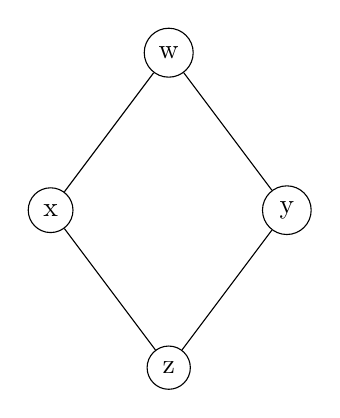
\begin{tikzpicture}[every node/.style={circle, draw, minimum size=0.25cm}]
      \node (w) at (0,2) {w};
      \node (y) at (-1.5,0) {x};
      \node (z) at (1.5,0) {y};
      \node (x) at (0,-2) {z};

      \draw (w) -- (y);
      \draw (w) -- (z);
      \draw (y) -- (x);
      \draw (z) -- (x);
    \end{tikzpicture}
    \subcaption{$\mathbf{A}$}
    \label{subfigure:partial-order-a}
  \end{subfigure}%
  \begin{subfigure}{0.3\textwidth}
    \centering
    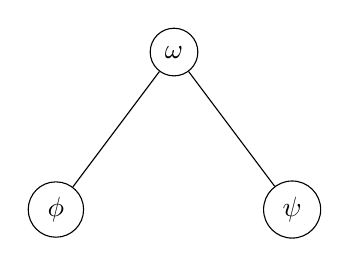
\begin{tikzpicture}[every node/.style={circle, draw, minimum size=0.25cm}]
      \node (y) at (-1.5,0) {$\phi$};
      \node (z) at (1.5,0) {$\psi$};
      \node (x) at (0,2) {$\omega$};

      \draw (y) -- (x);
      \draw (z) -- (x);
    \end{tikzpicture}
    \subcaption{$\mathbf{B}$}
    \label{subfigure:partial-order-b}
  \end{subfigure}%
  \caption{Hasse diagrams of two partially ordered sets}
  \label{figure:hasse-diagram}
\end{figure}

As an illustrative example, from the ordered set in \Cref{subfigure:partial-order-a} we read that $z \preceq x$, as there is a (strictly) upward path from $z$ to $x$. In fact, it is clear that $z \preceq w, x,y,z$, or that \say{$z$ is preferred to every other element in $\mathbf{A}$}. We say such an element is \textit{minimal}.

More formally, an element $x \in \mathbf{X}$ is \textit{minimal} with respect to the ordering if there exists no distinct element $y \in \mathbf{X}$ such that $y \preceq x$. Conversely, we say $x$ is \textit{maximal} if there exists no distinct $y \in \mathbf{X}$ where $x \preceq y$. Then $x$ is the \textit{minimum} element if $x \preceq y$ for all $y \in \mathbf{X}$; the dual notion of a \textit{maximum} is defined as we might expect. \index{maximum} \index{minimum} \index{maximal} \index{minimal}

\begin{definition}
  \label{definition:order-maps}
  \index{order-preserving map} \index{order-embedding} \index{order-isomorphism}
  Let $\mathbf{X}$ and $\mathbf{Y}$ be ordered sets with a mapping $\varphi : \mathbf{X} \to \mathbf{Y}$. We call $\varphi$ an \textit{order-preserving} (or, isotone) map if $x \preceq_X y$ implies $\varphi(x) \preceq_Y \varphi(y)$. It is an \textit{order-embedding} if it is injective, and $x \preceq_X y$ if and only if $\varphi(x) \preceq_Y \varphi(y)$ for all $x,y \in X$. Finally, $\varphi$ is an \textit{order-isomorphism} if it is an order-embedding that is also \textit{surjective}. The dual notion to an order-preserving map is an \textit{order-reversing} (or, antitone) map. \index{order-reversing map}
\end{definition}

\subsection{Lattice Theory}
\label{subsection:lattice-theory}
Lattice theory studies partially ordered sets that behave well with respect to upper and lower bounds. Given an ordered set $\mathbf{X}$ and a subset $\mathbf{Y} \subseteq \mathbf{X}$, the set of upper bounds of $\mathbf{Y}$ is defined as
\[
\mathbf{Y}^u \coloneqq \{x \in \mathbf{X} \mid \forall y \in \mathbf{Y} : y \preceq x\},
\]
and the set of lower bounds, $\mathbf{Y}^l$, is defined dually. If $\mathbf{Y}^u$ has a minimum element, then we call that element the \textit{supremum} of $\mathbf{Y}$; dually, if $\mathbf{Y}^l$ has a maximum element, then we call that element the \textit{infimum} of $\mathbf{Y}$. Instead of talking about the supremum of two elements $x,y \in \mathbf{X}$, we opt for the term \textit{join} and write $x \vee y$, or $\bigvee \mathbf{Y}$ where $\mathbf{Y} \subseteq \mathbf{X}$. Instead of infimum, we say \textit{meet} and write $x \wedge y$, or $\bigwedge \mathbf{Y}$. \index{upper bound} \index{lower bound} \index{join} \index{meet}

A \textit{lattice} is a non-empty partially ordered set $\mathbf{L}$ in which every pair of elements $x,y \in \mathbf{L}$ for which $x \wedge y$ and $x \vee y$ exists. If $\bigwedge \mathbf{M}$ and $\bigvee \mathbf{M}$ exist for any subset $\mathbf{M} \subseteq \mathbf{L}$ then $\mathbf{L}$ is a \textit{complete lattice}. \index{lattice} \index{lattice! complete lattice}

% \begin{example}
%   \label{example:lattice of naturals}
%   The set $\mathbb{N}$ of natural numbers forms a complete lattice when ordered by divisibility. In this lattice, the meet and join operations correspond to the greatest common divisor and least common multiple, respectively. The bottom element of the lattice is $1$, as it divides all natural numbers; while the top element is $0$ since it divides every natural.
% \end{example}

\subsubsection{Lattices as algebraic structures}
\label{subsubsection:lattices-as-algebraic-structures}

From another perspective, we can view lattices as an algebraic structure where meet and join are binary operations on the lattice. Then, $\langle L, \vee, \wedge \rangle$ is a lattice (although, we will just write $L$ and use the surrounding context as guidance). 

For each binary operation we have a substructure called a \textit{semilattice}. That is, $\langle L, \vee \rangle$ is a \textit{join semilattice} and $\langle L, \wedge \rangle$ is called a \textit{meet semilattice}. The $\vee$ operation of join semilattice $\langle L, \vee \rangle$ (resp. meet semilattice $\langle L, \wedge \rangle$) is
\vspace{-1em}
\begin{align}
     \text{(associative)} & \quad x \vee y = y \vee x & \text{(resp.)}  & \quad x \wedge y = y \wedge x \\
     \text{(commutative)} & \quad (x \vee y) \vee z = x \vee (y \vee z) & \quad \text{(resp.)} & (x \wedge y) \wedge z = x \wedge (y \wedge z) \\ 
     \text{(idempotent)}  & \quad x \vee x = x & \text{(resp.)}  & \quad x \wedge x = x
\end{align}
for all $x,y,z \in L$. 

The relationship between a lattice $\langle L, \vee, \wedge \rangle$ and its substructures $\langle L, \vee\rangle$ and $\langle L, \wedge \rangle$ is described by another property
\vspace{-1em}
\begin{align}
     \text{(absorbtion)} & \quad x \vee (x \wedge y) = x & \text{(resp.)}  & \quad x \wedge (x \vee y) = x 
\end{align}


\begin{lemma}[The Connecting Lemma]
  \label{lemma:the-connecting-lemma}
  If $\mathbf{L}$ is a lattice with $x, y \in \mathbf{L}$, then the following are equivalent:
  \begin{enumerate}
      \setlength\itemsep{0pt}
      \setlength\parsep{0pt}
    \item $x \preceq y$;
    \item $x \vee y = y$;
    \item $x \wedge y = x$.
  \end{enumerate}
\end{lemma}

